\pagestyle{ayllon}
\label{ayllon}


\begin{textblock*}{5.625in}(0pt,0pt)%
\vspace*{-3.2cm}
\hspace*{-1.95cm}\includegraphics*[width=145mm]{./imgs/AYLLON.png}
\end{textblock*}

\pagebreak %CABALAT SHABAT

\begin{center}
\hspace*{.5cm}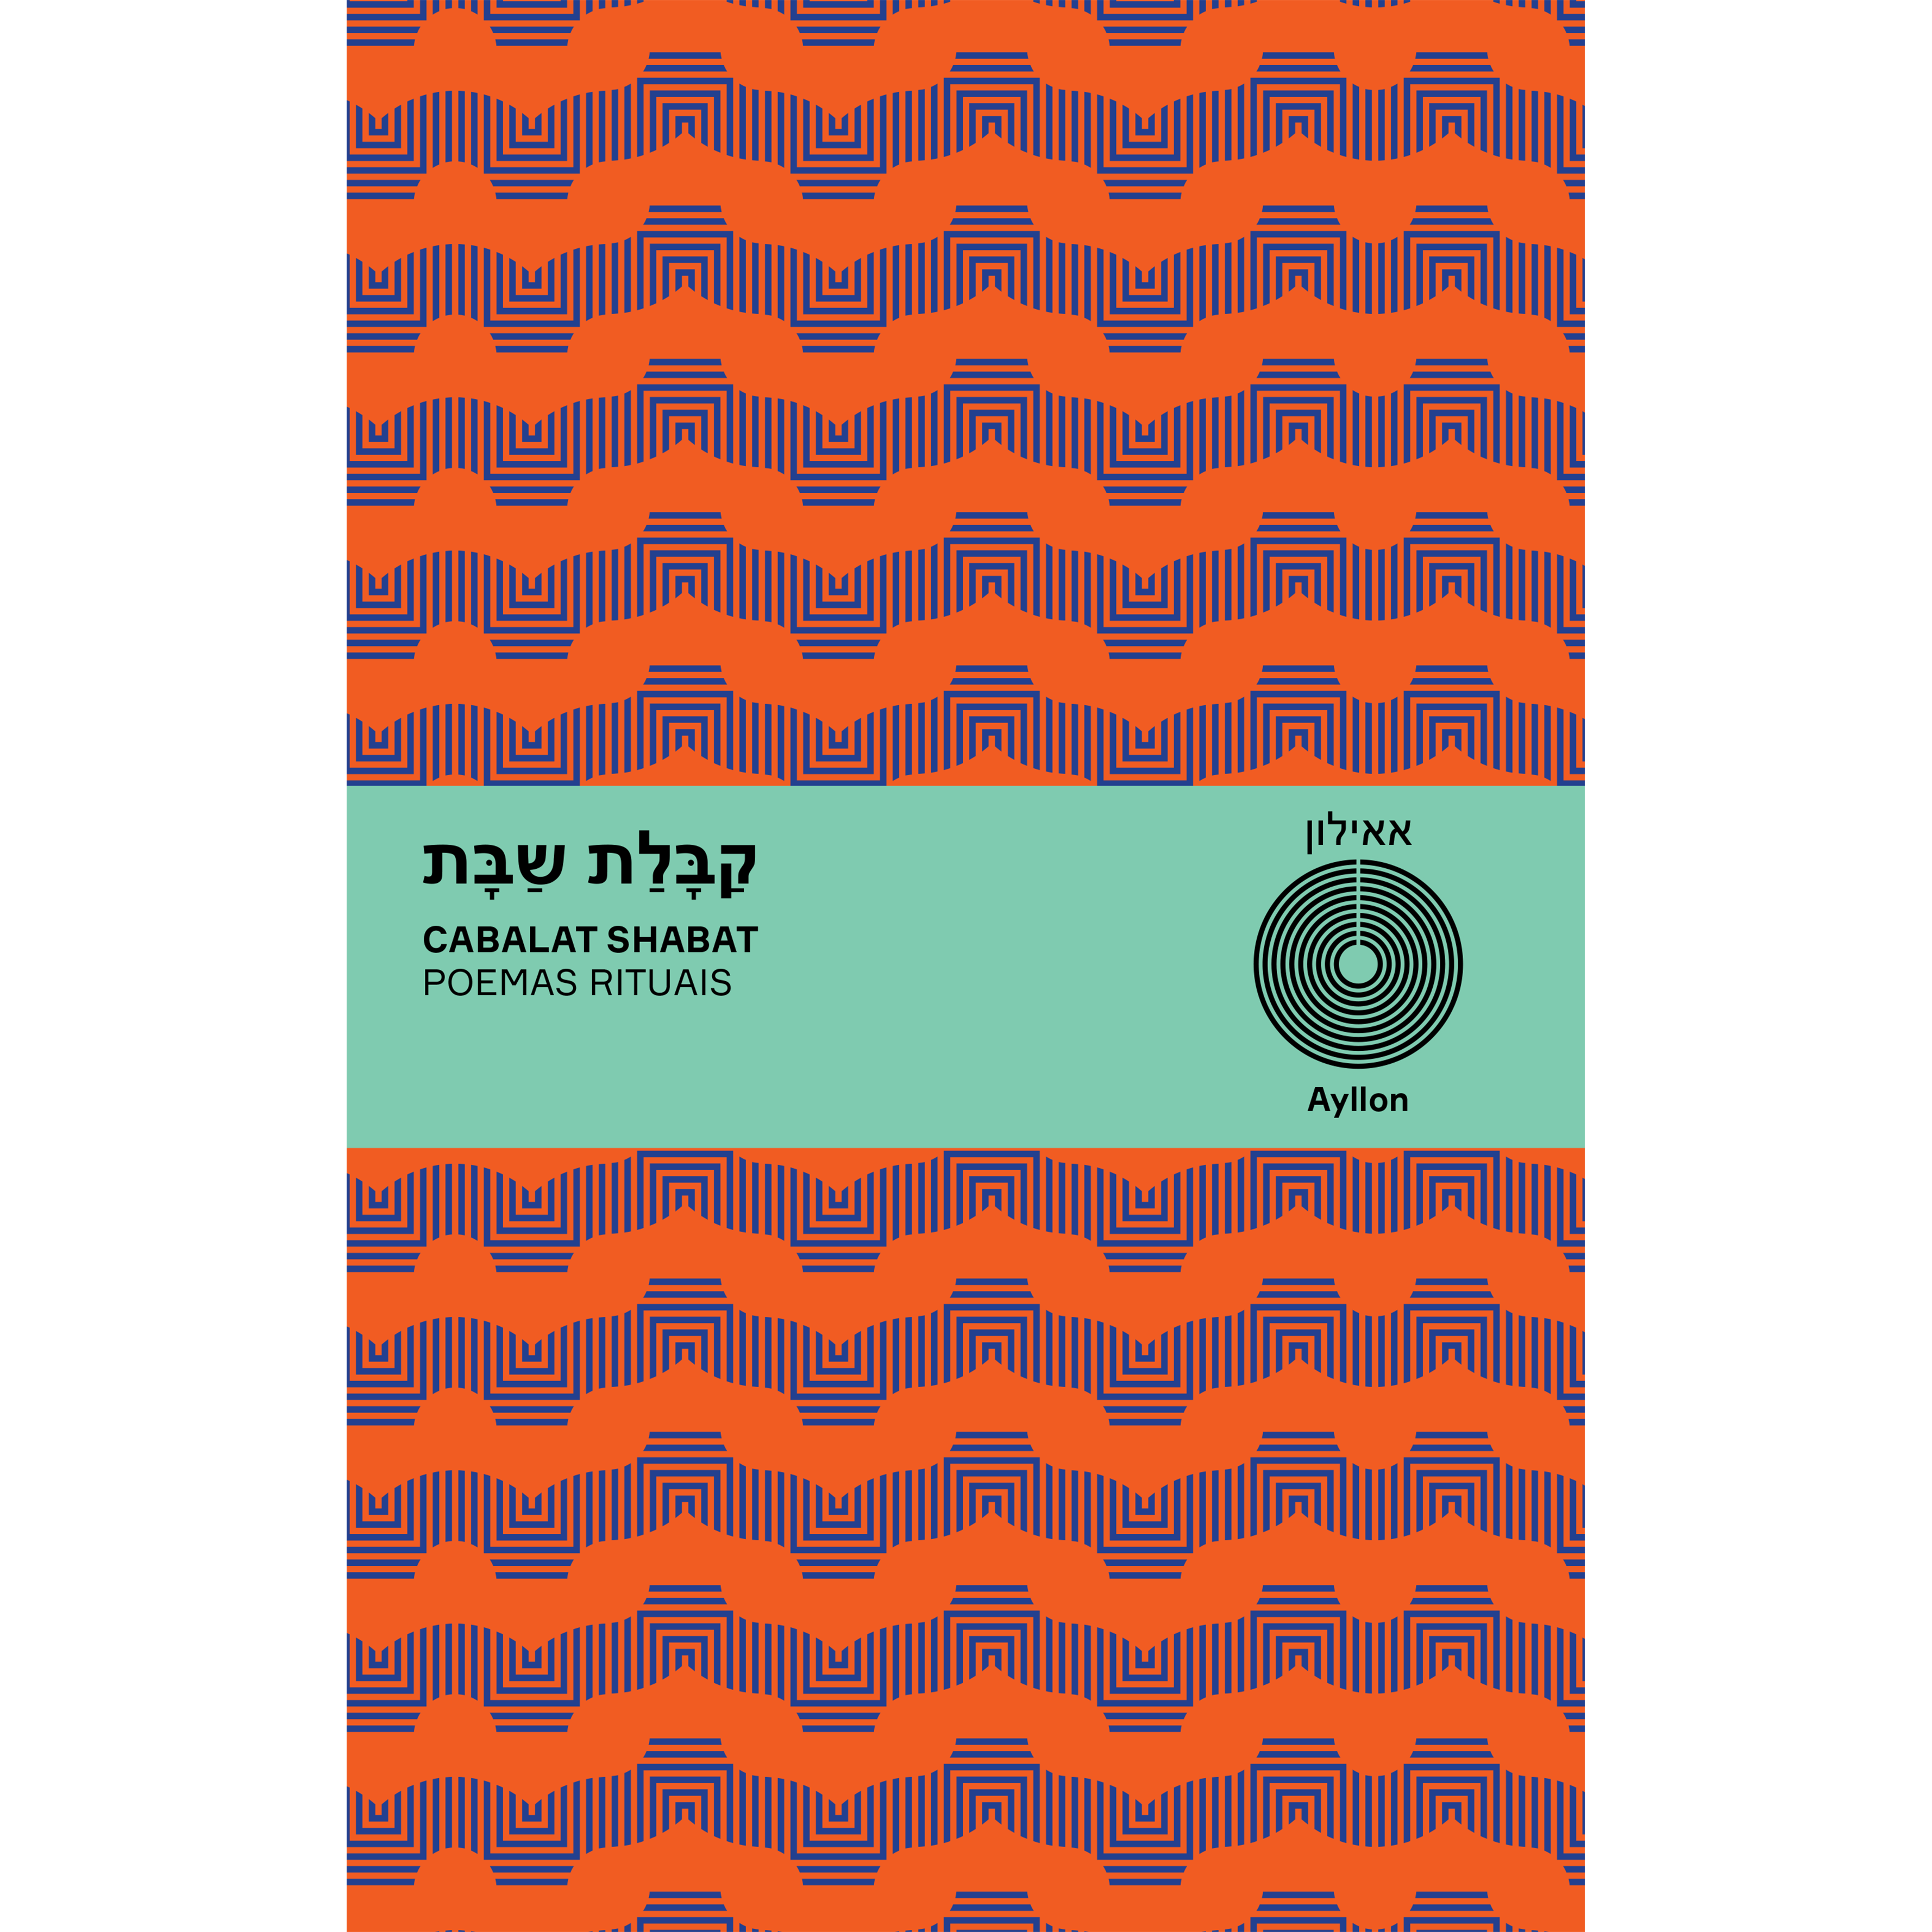
\includegraphics[width=74mm]{./grid/cabalat.png}
\end{center}

\hspace*{-7cm}\hrulefill\hspace*{-7cm}

\medskip

\noindent{}{\slsc{Cabalat shabat — poemas rituais}} é uma plaquete que reúne rezas e bênçãos judaicas entoadas na cerimônia de cabalat shabat, ou seja, no recebimento do shabat a partir do pôr"-do"-sol da sexta"-feira. Com alto teor místico e alusão à cabala, os textos nesta seleta são apresentados como poemas. E de maneira secular, mas não anti"-religiosa.

Em tradução direta do hebraico, a temática tratada no shabat --- a encenação da celebração do casamento entre Deus e o povo de Israel --- é situada paralelamente a outros lugares poéticos através do texto introdutório do volume, trazendo no próprio ritual um entendimento estrutural e histórico do judaísmo como simbologia. Em especial o antigo gênero grego epitalâmio (que vem de tálamo, ou quarto nupcial) e faz parte do cânone lírico. Através dessa ótica, é apresentada na leitura dos poemas um Deus mais próximo de quem o procura no âmbito doméstico, numa manobra alegórica que transforma um dos menos divinos gêneros em um lugar de comunhão.


\vfill

%\begin{wraptable}{l}{15cm}
\hspace*{-.4cm}\begin{minipage}[c]{.5\linewidth}
\small{
{\Formular{\textbf{
\hspace*{-.1cm}\hlc[lightyellow]{Editora: Ayllon}\\
Título: Cabalat Shabat — poemas rituais\\
Autor: Fabiana Grinberg (.org)\\ 
ISBN: 978-85-7715-610-8\\
Páginas: 28\\
Formato: 17,1x26,7cm\\
Preço: R\$ 29,90\\
Disponibilidade: 03/07/2020
}}}}
\end{minipage}
%\end{wraptable}


\pagebreak %FRAGMENTOS DE UM DIÁRIO ENCONTRADO

\begin{center}
\hspace*{-3.6cm}\raisebox{5cm}{\rotatebox[origin=t]{90}{\huge\Formular{\textbf{Lançamento}}}}
\hspace*{3.1cm}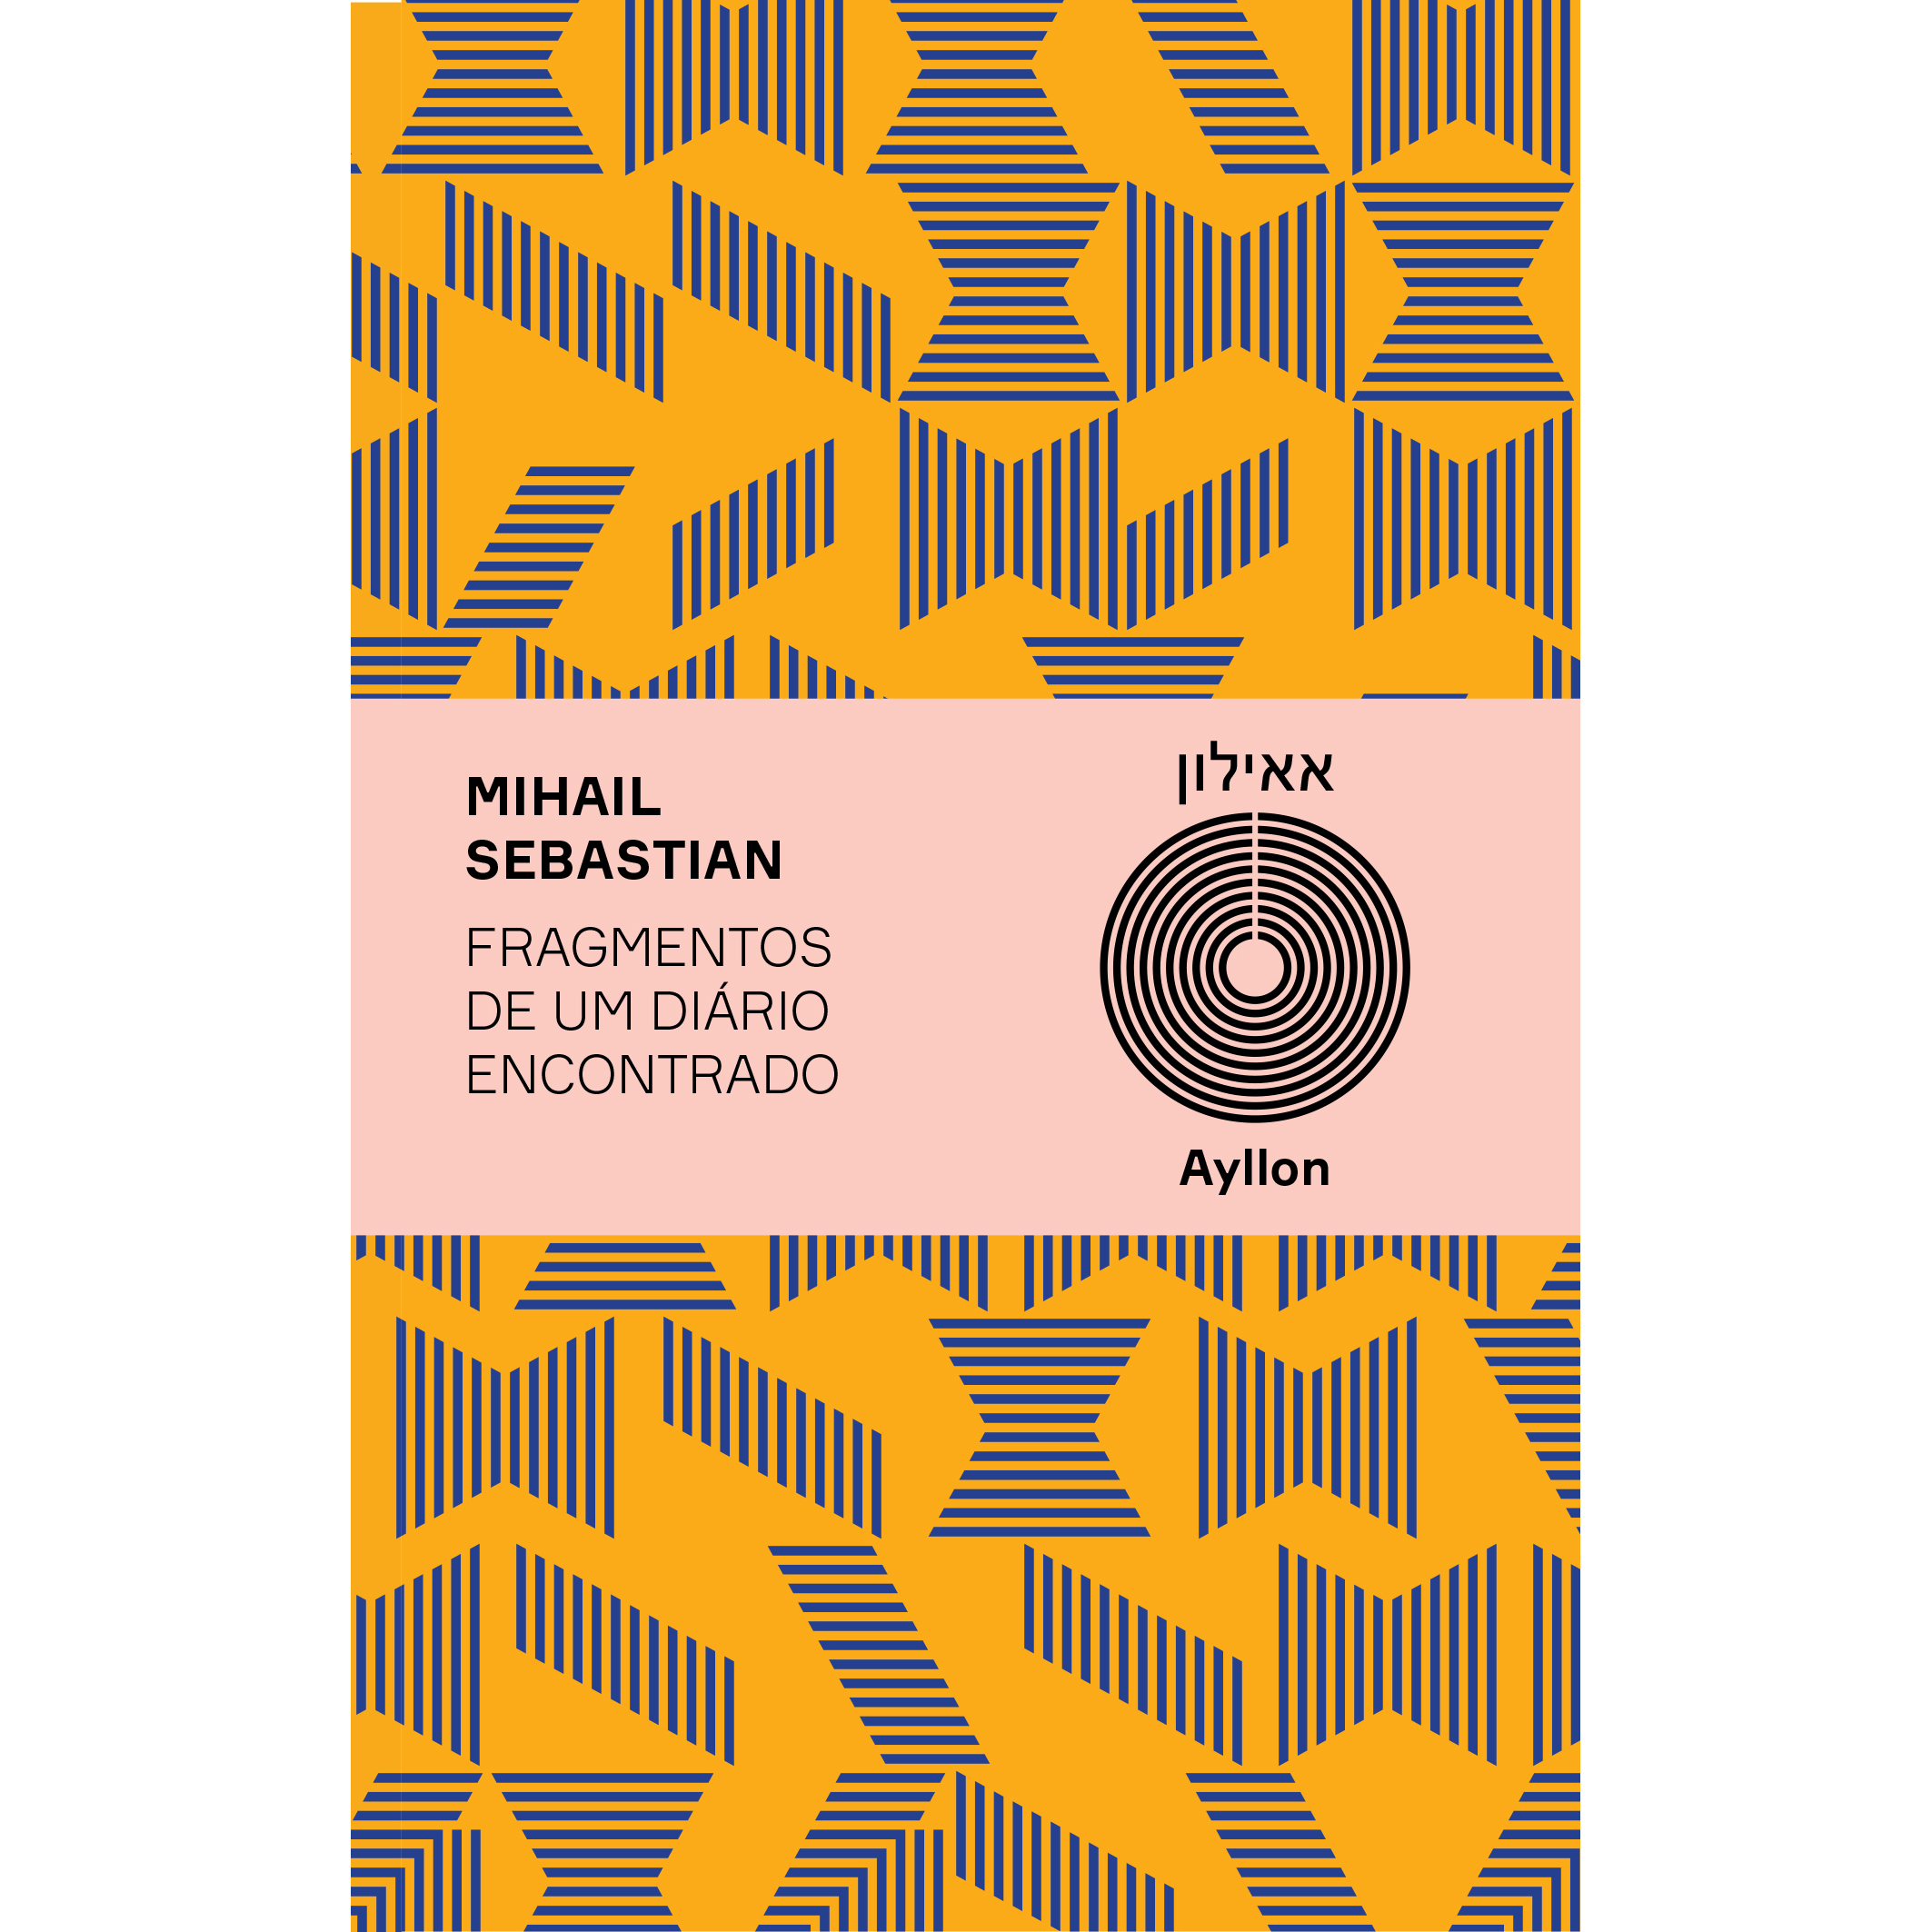
\includegraphics[width=74mm]{./grid/sebastian.jpg}
\end{center}

\hspace*{-7cm}\hrulefill\hspace*{-7cm}

\medskip

\noindent{}A narrativa de {\slsc{Fragmentos de um diário encontrado}} é escrita em torno da figura de alguém que se entrega aos labirintos de circulação urbana em busca de algo tão perdido quanto indefinível. O diário encontrado na ponte Mirabeau em Paris, segundo a (ficcional?) nota introdutória do volume, foi traduzido do francês para o romeno de forma desastrada. Através das passagens desse diário, o autor anônimo encarna o olhar do errante sobre a cidade.

A obra de 1932, escrita por Mihail Sebastian, é afinada com o caráter rebelde das vanguardas artísticas europeias das décadas de 1920 e 1930, que influenciaram o autor tanto quanto outros literatos compatriotas romenos de seu tempo --- como Cioran, Ionesco e Eliade. Judeu, Sebastian passou a ser excluído e execrado desse círculo. A publicação de {\slsc{Fragmentos de um diário encontrado}} traz de volta à atenção do público um autor importante no cenário literário romeno, injustamente excluído da posteridade tanto quanto o elusivo protagonista dessa narrativa.

\vfill

\hspace*{-.4cm}\begin{minipage}[c]{1\linewidth}
\small{
{\Formular{\textbf{
\hspace*{-.1cm}\hlc[lightyellow]{Editora: Ayllon}\\
Título: Fragmentos de um diário encontrado\\
Autor: Mihail Sebastian\\ 
ISBN: 978-85-7715-620-7\\
Páginas: 96\\
Formato: 11x18cm\\
Preço: R\$ 29,90\\
Disponibilidade: 03/07/2020
}}}}
\end{minipage}

\pagebreak

\vspace*{1.5cm}

\noindent{}{\nohyphens{\LARGE{Quem é Ayllon?\\\noindent{}{\large\slsc{O nome do novo selo da Hedra, dedicado a estudos judaicos,\\ vem de Salomon Ayllon, homem do século \scalebox{.8}{XVII}, que não poderia\\ ser facilmente classificado como uma figura religiosa ou secular}}}}}

\bigskip

\hfill{}\scalebox{.8}{SUZANA SALAMA}

\bigskip
\bigskip
\bigskip

Ayllon foi {\slsc{chacham}} [sábio, em hebraico], ou rabino de acordo com a tradição sefardita, das congregações de Londres e Amsterdã durante século \scalebox{.8}{XVII}. E embora tenha sido um religioso de posições polêmicas, não poderia ser classificado simplesmente como talmudista --- ou secular. Seguiu Sabatai Tzvi (1626--1676), mas não por longo tempo. Casou"-se com uma mulher informalmente divorciada, o que o levou a escrever uma carta aberta e polêmica sobre o assunto. Visitou vários países e comunidades judaicas pela Eupora e oriente como {\slsc{shaliach}} [emissário, em hebraico] da congregação palestina de Safed. Declarou inofensivas obras cabalísticas consideradas até então altamente heréticas. Deixou Londres por conta de suas divergências intelectuais, tendo sido acusado pela própria congregação sobre sua conduta. Escreveu uma obra sobre cabala, nunca publicada, mantida até hoje em manuscrito na Inglaterra. Sua figura é tão difícil de classificar como a do seu contemporâneo, Baruch Espinoza, que também não poderia ser classificado como secular --- ou talmudista.

Como sabemos, Espinoza, descendente de portugueses de Évora, foi expulso da comunidade judaica de Amsterdã em 1656, quando tinha 24 anos. E faleceu em 1677, 24 anos antes de Solomon Ayllon chegar a Amsterdã. Nunca se encontraram e nem poderiam, pois o {\slsc{chérem}} [maldição, em hebraico] contra Espinoza ordenava que ``ninguém lhe pode falar, nem por escrito, nem conceder"-lhe nenhum favor, nem debaixo do mesmo teto estar com ele, nem a uma distância de menos de quatro côvados, nem ler papel algum feito ou escrito por ele''. Baruch Espinoza foi um pensador livre, ousado, polêmico e radical à época, mas sua radicalidade foi produzida no enfrentamento a questões teológicas. Sua ideia de Deus como natureza, onde nada é intrinsecamente bom ou ruim, fez com que o marcassem como ateu ou panteísta. Desde que foi afastado da comunidade, recebeu diferentes rótulos durante os séculos. 

Como herege, Espinoza poderia ser o oposto do rabino Solomon Ayllon, que não fora expulso como ele. Mas não é. Ambos poderiam ser chamados humanistas, e por conta das convicções muito particulares sobre religião e sociedade foram censurados pela própria comunidade de diferentes formas. 

Frequentaram na Holanda a mesma biblioteca, ainda ativa atualmente, a {\slsc{Ets Haim}} --- ``Livraria Montezinos'', fundada pela comunidade portuguesa em 1616. Lá talvez tenham compulsado o mesmo exemplar de {\slsc{Puerta de cielo}}, do espanhol Abraham Cohen Herrera, discípulo do mestre cabalista Isaac Lúria. As anotações internas do livro (que une ensinamentos do Sefer Yetzirá, Zohar, escola luriânica e metafísica neoplatônica) dizem que deve ser mantido como uma jóia. Também segundo as notas, foi doado à Ets Haim pelo rabino Jacob Ferrares para preservação de possíveis usos impróprios no futuro. 

{\slsc{Puerta de cielo}} é um texto cabalístico impressionante e que fez parte da formação de Espinoza e Ayllon, entre tantos outros livros. O misticismo não apenas renova a tradição, mas preserva e dá novo significado. Pois na multiplicidade de interpretações dá"-se a santidade do texto, estabelecida justamente na capacidade de se desdobrar.

Nesse novo selo editorial, pretendemos que a tradição seja revisitada através do estudo, da crítica histórica, da filosofia e literatura judaicas, mas também dos ritos, discussões, mudanças, lugares, línguas, culturas, luzes, mistérios --- e sobretudo através de seu humanismo particular e significativo. Alegoricamente, as publicações que pretendemos publicar podem se perfazer como um encontro entre Ayllon e Espinoza, com a tradição e o enfrentamento, que fez parte de suas trajetórias. E a partir do logo, cujo símbolo cabalístico representa o {\slsc{Ein Sof}} [infinito, em hebraico], iniciamos o nosso novo projeto editorial.\footnote{Publicado originalmente no {\slsc{Medium}} da Hedra, em 6 de maio de 2020.}

\pagebreak
